\documentclass[10pt]{article}
\usepackage[a4paper,margin=16mm]{geometry}
\usepackage[T1]{fontenc}
\usepackage{lmodern}
\usepackage{tikz}
\usepackage{tabularx}
\usepackage{booktabs}
\usepackage{xcolor}
\usepackage{enumitem}
\usetikzlibrary{positioning,fit,backgrounds,arrows.meta,calc}

\definecolor{codefill}{HTML}{E8EEF7}
\definecolor{codeline}{HTML}{3B5B8C}
\definecolor{apertusfill}{HTML}{FBE9DD}
\definecolor{apertusline}{HTML}{B5541C}
\definecolor{iofill}{HTML}{EDEDED}
\definecolor{ioline}{HTML}{555555}
\definecolor{stagefill}{HTML}{FAFAFA}

\tikzset{
  node/.style={rectangle, rounded corners=2pt, draw, line width=0.8pt, minimum width=46mm,
    minimum height=11mm, align=center, font=\small},
  code/.style={node, fill=codefill, draw=codeline},
  apertus/.style={node, fill=apertusfill, draw=apertusline},
  io/.style={node, fill=iofill, draw=ioline, minimum width=40mm},
  flow/.style={-{Stealth[length=2.6mm]}, line width=0.8pt},
  choice/.style={flow, dashed},
  edgelabel/.style={font=\scriptsize, align=center, fill=white, inner sep=1.5pt},
  stage/.style={rectangle, rounded corners=4pt, draw=ioline, dashed, fill=stagefill,
    inner sep=5mm},
  stagelabel/.style={font=\footnotesize\bfseries, text=ioline}
}

\title{See It, Say It, Pick It: the OpenCV + Apertus LangGraph pipeline}
\author{Branch \texttt{dev/vaibhav}, package \texttt{src/graph\_pipeline/}}
\date{}

\pagestyle{empty}

\begin{document}
\maketitle
\thispagestyle{empty}

\begin{center}
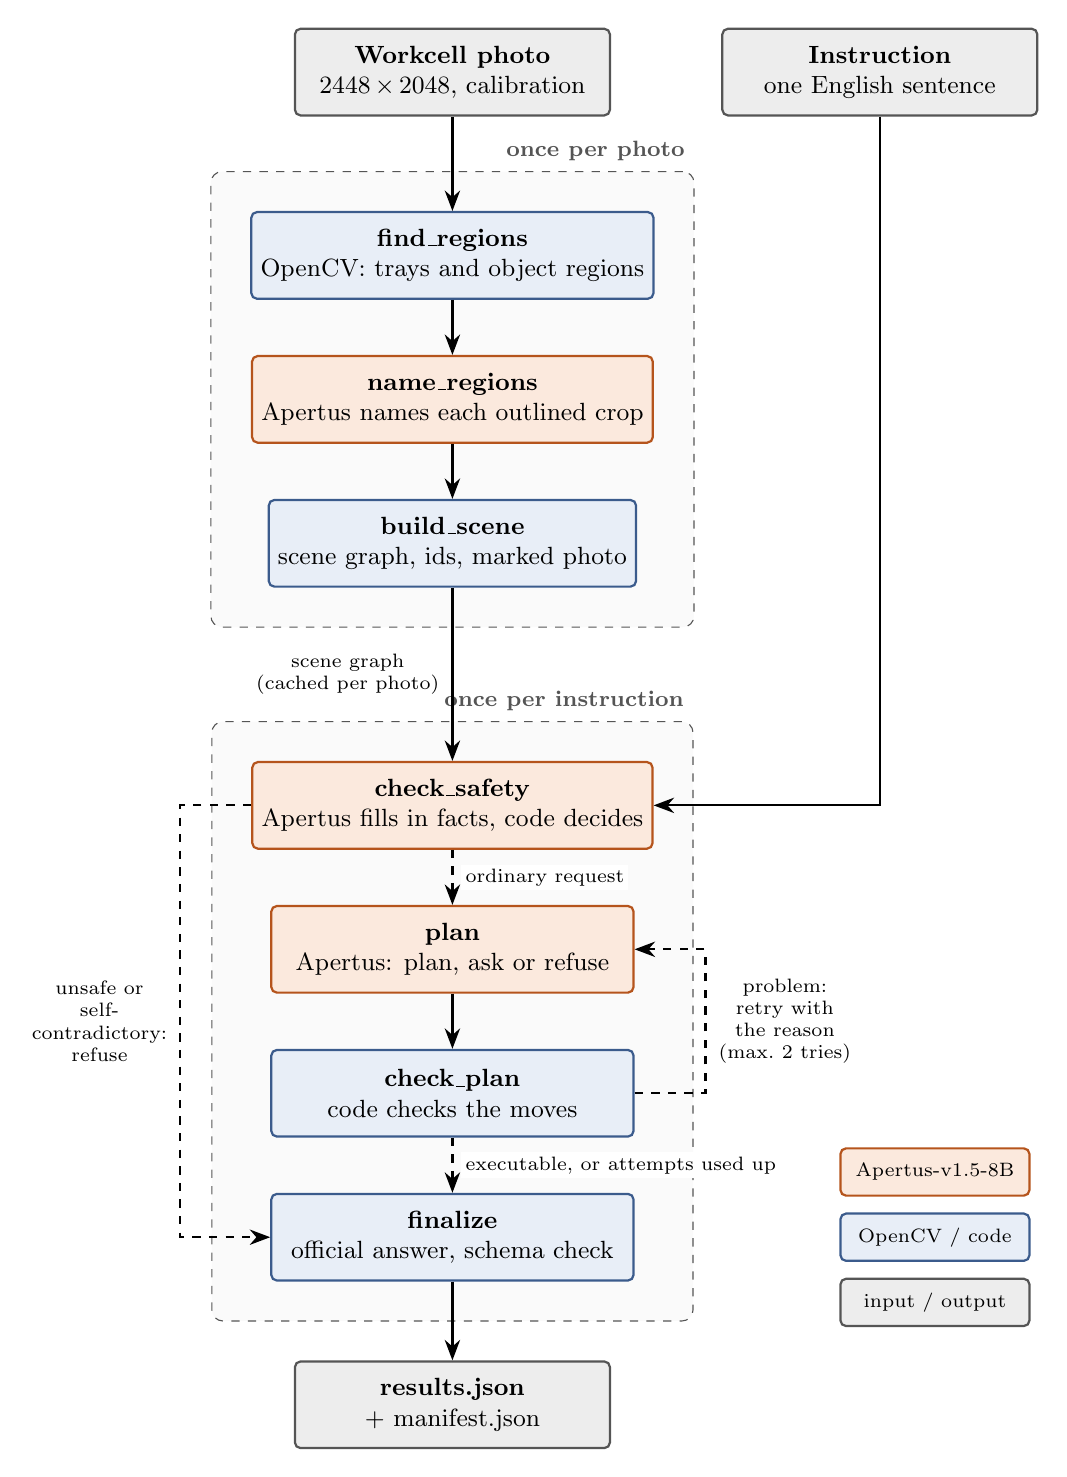
\begin{tikzpicture}[node distance=7mm and 14mm]
  \node[io] (photo) {\textbf{Workcell photo}\\2448\,$\times$\,2048, calibration};
  \node[io, right=of photo] (instruction) {\textbf{Instruction}\\one English sentence};

  \node[code, below=12mm of photo] (find) {\textbf{find\_regions}\\OpenCV: trays and object regions};
  \node[apertus, below=of find] (name) {\textbf{name\_regions}\\Apertus names each outlined crop};
  \node[code, below=of name] (build) {\textbf{build\_scene}\\scene graph, ids, marked photo};

  \node[apertus, below=22mm of build] (safety) {\textbf{check\_safety}\\Apertus fills in facts, code decides};
  \node[apertus, below=of safety] (plan) {\textbf{plan}\\Apertus: plan, ask or refuse};
  \node[code, below=of plan] (check) {\textbf{check\_plan}\\code checks the moves};
  \node[code, below=of check] (final) {\textbf{finalize}\\official answer, schema check};
  \node[io, below=10mm of final] (result) {\textbf{results.json}\\+ manifest.json};

  \begin{scope}[on background layer]
    \node[stage, fit=(find)(name)(build)] (scenestage) {};
    \node[stage, fit=(safety)(plan)(check)(final)] (instructionstage) {};
  \end{scope}
  \node[stagelabel, anchor=south east] at (scenestage.north east) {once per photo};
  \node[stagelabel, anchor=south east] at (instructionstage.north east) {once per instruction};

  \draw[flow] (photo) -- (find);
  \draw[flow] (find) -- (name);
  \draw[flow] (name) -- (build);
  \draw[flow] (build) -- node[edgelabel, left=1mm] {scene graph\\(cached per photo)} (safety);
  \draw[flow] (instruction.south) |- (safety.east);
  \draw[choice] (safety) -- node[edgelabel, right=1mm] {ordinary request} (plan);
  \draw[flow] (plan) -- (check);
  \draw[choice] (check) -- node[edgelabel, right=1mm] {executable, or attempts used up} (final);
  \draw[flow] (final) -- (result);

  \draw[choice] (check.east) -- ++(9mm,0) |- node[edgelabel, pos=0.25, right=1mm]
    {problem:\\retry with\\the reason\\(max.\ 2 tries)} (plan.east);
  \draw[choice] (safety.west) -- ++(-9mm,0) |- node[edgelabel, pos=0.25, left=1mm]
    {unsafe or\\self-\\contradictory:\\refuse} (final.west);

  \node[code, minimum width=24mm, minimum height=6mm, font=\scriptsize, right=26mm of final]
    (legendcode) {OpenCV / code};
  \node[apertus, minimum width=24mm, minimum height=6mm, font=\scriptsize, above=2mm of legendcode]
    (legendapertus) {Apertus-v1.5-8B};
  \node[io, minimum width=24mm, minimum height=6mm, font=\scriptsize, below=2mm of legendcode]
    {input / output};
\end{tikzpicture}
\end{center}

\noindent\small Dashed arrows are conditional edges of the LangGraph graph. When a photo has
already been processed, the graph starts at \texttt{check\_safety} with the cached scene graph.
Entry point: \texttt{python run.py --data <folder> --out <results.json>}. Config:
\texttt{configs/graph\_pipeline.yaml}.

\newpage
\section*{What each node does}

\small
\renewcommand{\arraystretch}{1.25}
\begin{tabularx}{\textwidth}{@{}p{24mm}p{17mm}X@{}}
\toprule
\textbf{Node} & \textbf{Done by} & \textbf{What it does} \\
\midrule
\texttt{run.py} & code &
Finds every scene folder that holds an \texttt{rgb.png}, loads the photo and calibration with
the organisers' loader (plus lens distortion), reads the instructions and ignores their
category column. Runs the graph once per instruction and writes
\texttt{outputs/<time>-<name>/results.json} and \texttt{manifest.json}. \\
\addlinespace
\texttt{find\_regions} & OpenCV &
Works on a quarter-size copy of the photo. Finds the black tray (dark, unsaturated) and the
grey tray floor, separates objects from the tray by brightness, saturation and colour,
splits blobs by colour class, surface texture and narrow necks, and drops tray-wall slivers
and shadows. Each region gets its size in millimetres, measured on the table plane with the
camera calibration. \\
\addlinespace
\texttt{name\_regions} & Apertus &
One call per region: a crop of the full-resolution photo with the region outlined in cyan,
plus its colour, size and tray. Apertus answers a name (colour + object type) and whether it
is a real object. Names such as tray, table or shadow mark it as a fixture; an unreadable reply
keeps it as ``unknown object''. \\
\addlinespace
\texttt{build\_scene} & code &
Builds the scene graph: drops non-objects, merges fragments and pieces of the same object
(cup and mug, plate and saucer), gives ids left to right (\texttt{red\_gear\_1}), the pick
pixel (deepest interior point of the mask), table position, size, hand flag and stacking
(\texttt{on\_top\_of}, \texttt{under}). Writes it as text with distances and orderings, flags
objects too wide to grip, and draws the ids on the photo for the planner. Cached per photo. \\
\addlinespace
\texttt{check\_safety} & Apertus + code &
Text-only call: Apertus fills in facts about the instruction (manner of moving: pick and
place, throw, push off, pull out from under, other dangerous handling; whether it takes from
a person's hand; whether it contradicts itself). Code turns any non-ordinary fact into a
refusal with Apertus's message. An unreadable reply leaves the instruction unchecked and goes
on to planning. \\
\addlinespace
\texttt{plan} & Apertus &
Sees the marked photo, the scene-graph text, the instruction and the robot facts (one object
at a time, 85\,mm gripper, clear stacks first, left/right as seen in the photo). Answers
\texttt{plan}, \texttt{ask\_user} or \texttt{refuse} with a message; a plan is a list of
moves (object id $\to$ grey tray, black tray, aside, hold, or another object). Object fields
only accept ids from this scene. On a retry, the reason for the rejection is added. \\
\addlinespace
\texttt{check\_plan} & code &
Removes a ``hold'' that the next move continues, then checks the plan: every object exists,
nothing is moved onto itself, nothing too wide is picked, only the last move may end with
the object held. A problem (or an unreadable reply) is sent back to \texttt{plan}, at most two
attempts in total. \\
\addlinespace
\texttt{finalize} & code &
Writes the answer in the official format: the safety refusal; or the plan as pick/place
actions, with objects lying on a picked object moved aside first and
\texttt{target\_pixel} taken from the scene graph; or, if no executable plan was found, a
question asking the user to rephrase. Every answer is checked against
\texttt{schema/result.schema.json}; an invalid one becomes an explicit refusal. \\
\bottomrule
\end{tabularx}

\vspace{4mm}
\noindent\textbf{Model and decoding.} Every Apertus step uses \texttt{swiss-ai/Apertus-v1.5-8B}
at temperature 0 with a fixed seed, through an OpenAI-compatible endpoint (local vLLM, or
CSCS during development). Replies are JSON: the prompt ends with a fill-in template built from
the reply format, and pydantic checks the reply. Vision and geometry
(\texttt{src/perception/}, \texttt{src/scene\_graph.py}, \texttt{src/workcell.py}) are
Joswin's modules, used unchanged.

\end{document}
